% figures/clinic-room-overlap.tex
\documentclass[11pt]{article}
\usepackage[margin=1.5cm]{geometry}
\usepackage{tikz}
\usetikzlibrary{arrows.meta}
\pagestyle{empty}
\begin{document}
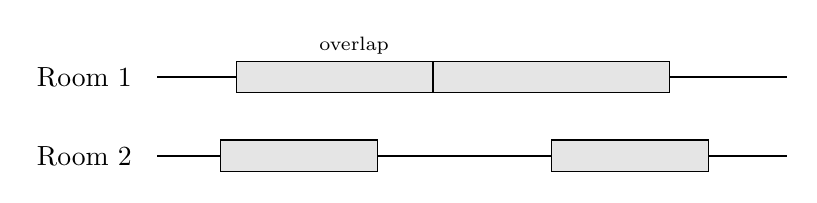
\begin{tikzpicture}[>=Latex]
  \node[anchor=east] at (-0.2,1.0) {Room 1};
  \node[anchor=east] at (-0.2,0.0) {Room 2};

  \draw[thick] (0,1.0) -- (8,1.0);
  \draw[thick] (0,0.0) -- (8,0.0);

  \draw[fill=gray!20] (1,0.8) rectangle (4,1.2);
  \draw[fill=gray!20] (3.5,0.8) rectangle (6.5,1.2);

  \draw[fill=gray!20] (0.8,-0.2) rectangle (2.8,0.2);
  \draw[fill=gray!20] (5.0,-0.2) rectangle (7.0,0.2);

  \node[font=\scriptsize] at (2.5,1.4) {overlap};
\end{tikzpicture}
\end{document}
